\documentclass[12pt,a4paper]{article}
\usepackage[utf8]{inputenc}
\usepackage[T1]{fontenc}
\usepackage{graphicx}
\usepackage{hyperref}
\usepackage{geometry}
\usepackage{setspace}
\usepackage{xcolor}
\usepackage{titlesec}
\usepackage{enumitem}
\usepackage{fancyhdr}
\usepackage{tikz}
\usepackage{tikz-3dplot}
\usetikzlibrary{shapes,arrows,positioning,fit,backgrounds,calc,shadows}
\usepackage{float}

% Layout
\geometry{margin=1in}
\setstretch{1.15}
\pagestyle{fancy}
\fancyhf{}
\rhead{\textbf{Federated ICS Engine – Architecture}}
\lhead{System Architecture Document}
\rfoot{\thepage}

% Section formatting
\titleformat{\section}{\large\bfseries\color{blue!60!black}}{\thesection.}{1em}{}
\titleformat{\subsection}{\bfseries\color{black}}{\thesubsection}{1em}{}
\titleformat{\subsubsection}{\bfseries\color{gray}}{\thesubsubsection}{1em}{}

\begin{document}

\begin{center}
    \vspace*{0.5cm}
    {\Huge \textbf{Federated ICS Threat Correlation Engine}}\\[0.4cm]
    {\LARGE System Architecture Document}\\[0.3cm]
    {\large Version 1.0}\\[0.2cm]
    \textit{Industrial Control Systems Security Team}\\[0.1cm]
    \textbf{Date:} \today\\
    \vspace{0.5cm}
\end{center}

\tableofcontents
\newpage

\section{Executive Summary}

This document provides a comprehensive architectural specification for the Federated ICS Threat Correlation Engine.
The system is designed to provide real-time threat detection, attack prediction, and privacy-preserving collaborative defense for industrial control systems across multiple facilities.


\subsection{Key Architectural Goals}

\begin{enumerate}[leftmargin=1cm,itemsep=0pt]
    \item \textbf{Real-Time Detection:} Detect threats within 30 seconds
    \item \textbf{High Accuracy:} >95\% detection accuracy, <5\% false positives
    \item \textbf{Privacy-Preserving:} Mathematical privacy guarantees (ε=2.0, δ=10⁻⁵)
    \item \textbf{Scalability:} Support 10-1000+ facilities
    \item \textbf{Resilience:} Byzantine-robust against malicious participants
    \item \textbf{Modularity:} Loosely coupled components for maintainability
\end{enumerate}

\subsection{Design Principles}

\textbf{1. Defense in Depth:} Multiple layers of security (network, application, data)

\textbf{2. Privacy by Design:} Data never leaves facility, privacy at every layer

\textbf{3. Fail-Safe:} System degrades gracefully under attack or failure

\textbf{4. Observable:} Comprehensive monitoring and logging

\textbf{5. Scalable:} Horizontal scaling for all components

\textbf{6. Standards-Based:} Use industry-standard protocols and frameworks

\section{System Overview}

\subsection{High-Level Architecture}

The system consists of six primary layers working together to provide comprehensive threat detection and collaborative defense.

\begin{figure}[H]
\centering
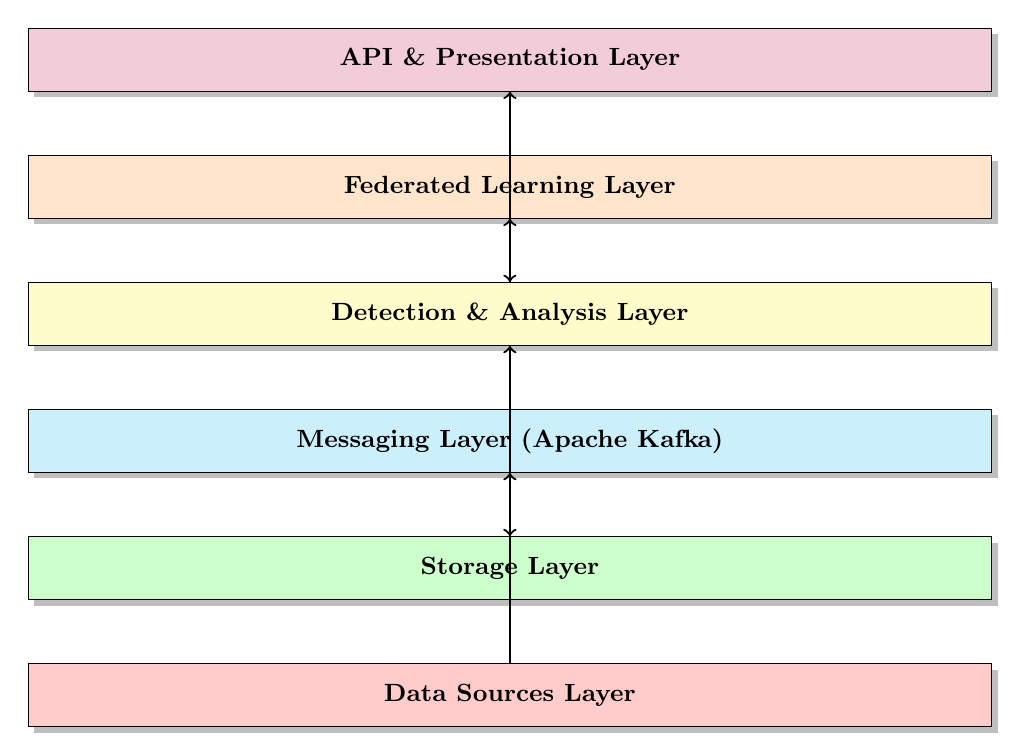
\begin{tikzpicture}[
    node distance=0.8cm,
    layer/.style={rectangle, draw, fill=blue!20, text width=12cm, align=center, minimum height=0.8cm, font=\bfseries\small, drop shadow}
]

% Layers from top to bottom
\node[layer, fill=purple!20] (api) {API \& Presentation Layer};
\node[layer, below=of api, fill=orange!20] (fl) {Federated Learning Layer};
\node[layer, below=of fl, fill=yellow!20] (detection) {Detection \& Analysis Layer};
\node[layer, below=of detection, fill=cyan!20] (messaging) {Messaging Layer (Apache Kafka)};
\node[layer, below=of messaging, fill=green!20] (storage) {Storage Layer};
\node[layer, below=of storage, fill=red!20] (sources) {Data Sources Layer};

% Arrows showing data flow
\draw[->, thick] (sources) -- (messaging);
\draw[->, thick] (messaging) -- (detection);
\draw[->, thick] (detection) -- (storage);
\draw[->, thick] (detection) -- (fl);
\draw[->, thick] (fl) -- (api);
\draw[->, thick] (api) -- (detection);

\end{tikzpicture}
\caption{High-Level System Architecture - Six-Layer Design}
\end{figure}


\subsection{Architecture Layers}

\subsubsection{Layer 1: Data Sources Layer}

Ingests data from industrial control systems:
\begin{itemize}[leftmargin=1cm,itemsep=0pt]
    \item Industrial protocols (Modbus, DNP3, OPC-UA, S7)
    \item Network traffic (pcap, NetFlow)
    \item SCADA logs and events
    \item Physical sensor readings
\end{itemize}

\subsubsection{Layer 2: Storage Layer}

Polyglot persistence for different data types:
\begin{itemize}[leftmargin=1cm,itemsep=0pt]
    \item \textbf{Apache IoTDB:} Time-series sensor data
    \item \textbf{PostgreSQL:} Alerts, incidents, metadata
    \item \textbf{MongoDB:} Logs, protocol messages
    \item \textbf{Neo4j:} Attack graphs, MITRE ATT\&CK relationships
\end{itemize}

\subsubsection{Layer 3: Messaging Layer}

Apache Kafka message bus:
\begin{itemize}[leftmargin=1cm,itemsep=0pt]
    \item Decouples producers and consumers
    \item High-throughput data streaming
    \item Message persistence and replay
    \item Topic-based routing
\end{itemize}

\subsubsection{Layer 4: Detection \& Analysis Layer}

Core threat detection components:
\begin{itemize}[leftmargin=1cm,itemsep=0pt]
    \item LSTM Autoencoder (behavioral anomalies)
    \item Isolation Forest (point anomalies)
    \item Physics Rules Engine (process violations)
    \item Protocol Anomaly Detection
    \item Correlation Engine (multi-source fusion)
    \item Attack Prediction GNN
\end{itemize}

\subsubsection{Layer 5: Federated Learning Layer}

Collaborative learning infrastructure:
\begin{itemize}[leftmargin=1cm,itemsep=0pt]
    \item FL Client (local training)
    \item FL Server (aggregation)
    \item Privacy Engine (differential privacy)
    \item Secure Aggregation
    \item Byzantine-Robust Aggregation
\end{itemize}

\subsubsection{Layer 6: API \& Presentation Layer}

External interfaces:
\begin{itemize}[leftmargin=1cm,itemsep=0pt]
    \item REST API (CRUD operations)
    \item GraphQL API (flexible queries)
    \item WebSocket (real-time updates)
    \item Web Dashboard (React)
    \item Mobile App (future)
\end{itemize}


\section{Detailed Component Architecture}

\subsection{Data Sources Layer Components}

\begin{figure}[H]
\centering
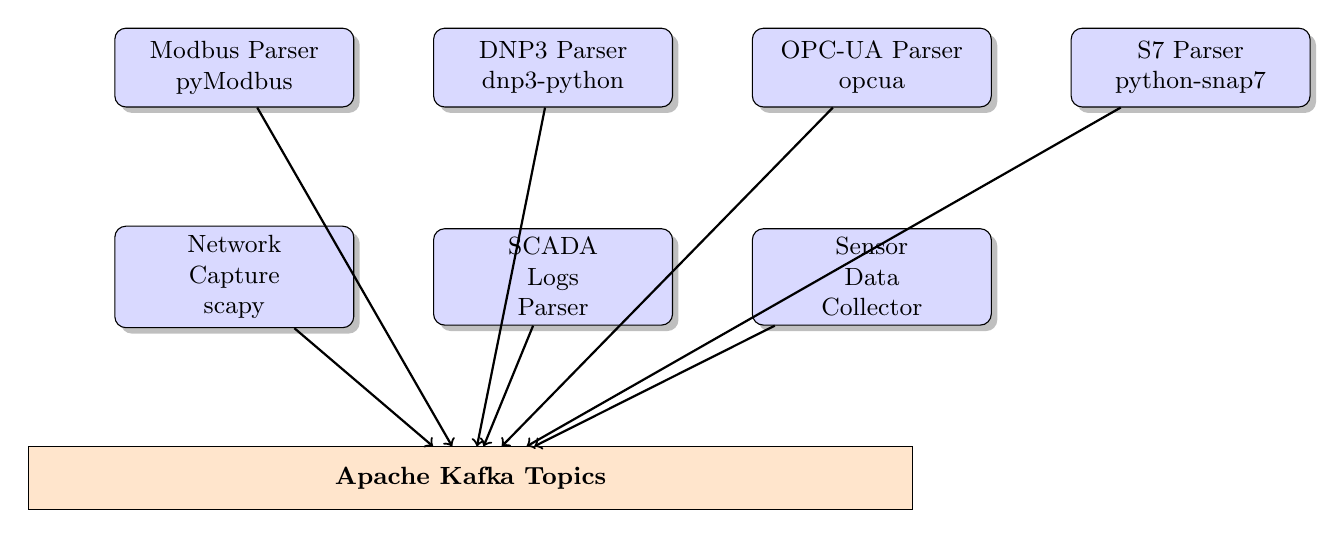
\begin{tikzpicture}[
    node distance=1cm,
    component/.style={rectangle, draw, fill=blue!15, text width=2.8cm, align=center, minimum height=1cm, rounded corners, font=\small, drop shadow},
    kafka/.style={rectangle, draw, fill=orange!20, text width=11cm, align=center, minimum height=0.8cm, font=\bfseries\small}
]

\node[component] (modbus) {Modbus Parser\\pyModbus};
\node[component, right=of modbus] (dnp3) {DNP3 Parser\\dnp3-python};
\node[component, right=of dnp3] (opcua) {OPC-UA Parser\\opcua};
\node[component, right=of opcua] (s7) {S7 Parser\\python-snap7};

\node[component, below=1.5cm of modbus] (pcap) {Network\\Capture\\scapy};
\node[component, right=of pcap] (scada) {SCADA\\Logs\\Parser};
\node[component, right=of scada] (sensors) {Sensor\\Data\\Collector};

\node[kafka, below=1.5cm of pcap, xshift=3cm] (kafka) {Apache Kafka Topics};

\draw[->, thick] (modbus) -- (kafka);
\draw[->, thick] (dnp3) -- (kafka);
\draw[->, thick] (opcua) -- (kafka);
\draw[->, thick] (s7) -- (kafka);
\draw[->, thick] (pcap) -- (kafka);
\draw[->, thick] (scada) -- (kafka);
\draw[->, thick] (sensors) -- (kafka);

\end{tikzpicture}
\caption{Data Sources Layer - Protocol Parsers and Collectors}
\end{figure}

\subsubsection{Protocol Parser: Modbus}

\textbf{Purpose:} Parse Modbus TCP/RTU protocol messages

\textbf{Responsibilities:}
\begin{itemize}[leftmargin=1cm,itemsep=0pt]
    \item Decode Modbus frames
    \item Extract function codes, addresses, values
    \item Detect malformed messages
    \item Publish to Kafka topic: \texttt{protocol.modbus}
\end{itemize}

\textbf{Technology:} Python 3.11+, pyModbus library

\subsubsection{Protocol Parser: DNP3}

\textbf{Purpose:} Parse DNP3 protocol (common in utilities)

\textbf{Responsibilities:}
\begin{itemize}[leftmargin=1cm,itemsep=0pt]
    \item Decode DNP3 frames
    \item Extract object variations, points
    \item Handle fragmentation
    \item Publish to Kafka topic: \texttt{protocol.dnp3}
\end{itemize}

\textbf{Technology:} Python 3.11+, dnp3-python

\textbf{Key Features:}
\begin{itemize}[leftmargin=1cm,itemsep=0pt]
    \item Master/Outstation communication
    \item Unsolicited response handling
    \item Integrity polls and event scans
\end{itemize}


\subsubsection{Protocol Parser: OPC-UA}

\textbf{Purpose:} Parse OPC-UA protocol (modern industrial standard)

\textbf{Responsibilities:}
\begin{itemize}[leftmargin=1cm,itemsep=0pt]
    \item Connect to OPC-UA servers
    \item Subscribe to data changes
    \item Monitor method calls
    \item Publish to Kafka topic: \texttt{protocol.opcua}
\end{itemize}

\textbf{Technology:} Python 3.11+, opcua library

\textbf{Security Features:}
\begin{itemize}[leftmargin=1cm,itemsep=0pt]
    \item Certificate-based authentication
    \item Encrypted communication
    \item User access control monitoring
\end{itemize}

\subsubsection{Network Capture Component}

\textbf{Purpose:} Capture and analyze network traffic

\textbf{Responsibilities:}
\begin{itemize}[leftmargin=1cm,itemsep=0pt]
    \item Packet capture (pcap)
    \item Protocol identification
    \item Flow analysis
    \item Anomaly detection (port scans, unusual connections)
    \item Publish to Kafka topic: \texttt{network.traffic}
\end{itemize}

\textbf{Technology:} Python 3.11+, scapy, tcpdump

\textbf{Capture Modes:}
\begin{itemize}[leftmargin=1cm,itemsep=0pt]
    \item \textbf{Always-on:} Metadata only (headers, flow stats)
    \item \textbf{Triggered:} Full packet capture on suspicious activity
\end{itemize}

\subsection{Messaging Layer: Apache Kafka}

\subsubsection{Architecture}

\begin{figure}[H]
\centering
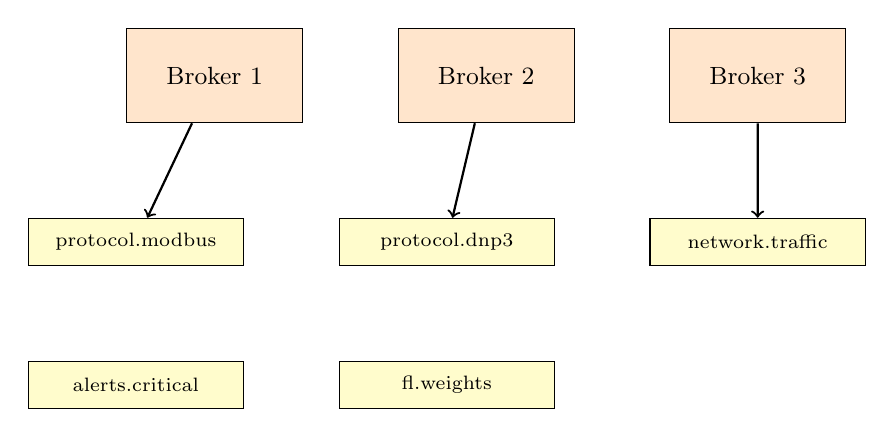
\begin{tikzpicture}[
    node distance=1.2cm,
    broker/.style={rectangle, draw, fill=orange!20, text width=2cm, align=center, minimum height=1.2cm, font=\small},
    topic/.style={rectangle, draw, fill=yellow!20, text width=2.5cm, align=center, minimum height=0.6cm, font=\scriptsize}
]

\node[broker] (b1) {Broker 1};
\node[broker, right=of b1] (b2) {Broker 2};
\node[broker, right=of b2] (b3) {Broker 3};

\node[topic, below=of b1, xshift=-1cm] (t1) {protocol.modbus};
\node[topic, right=of t1] (t2) {protocol.dnp3};
\node[topic, right=of t2] (t3) {network.traffic};
\node[topic, below=of t1] (t4) {alerts.critical};
\node[topic, right=of t4] (t5) {fl.weights};

\draw[->, thick] (b1) -- (t1);
\draw[->, thick] (b2) -- (t2);
\draw[->, thick] (b3) -- (t3);

\end{tikzpicture}
\caption{Kafka Cluster Architecture - 3 Brokers, Multiple Topics}
\end{figure}

\textbf{Purpose:} High-throughput message bus for system-wide communication

\textbf{Key Features:}
\begin{itemize}[leftmargin=1cm,itemsep=0pt]
    \item Distributed, fault-tolerant
    \item Horizontal scalability
    \item Message persistence (configurable retention)
    \item Exactly-once semantics
    \item Consumer groups for load balancing
\end{itemize}


\subsection{Detection \& Analysis Layer}

\subsubsection{LSTM Autoencoder Component}

\textbf{Purpose:} Detect behavioral anomalies in time-series data

\textbf{Architecture:}

\begin{figure}[H]
\centering
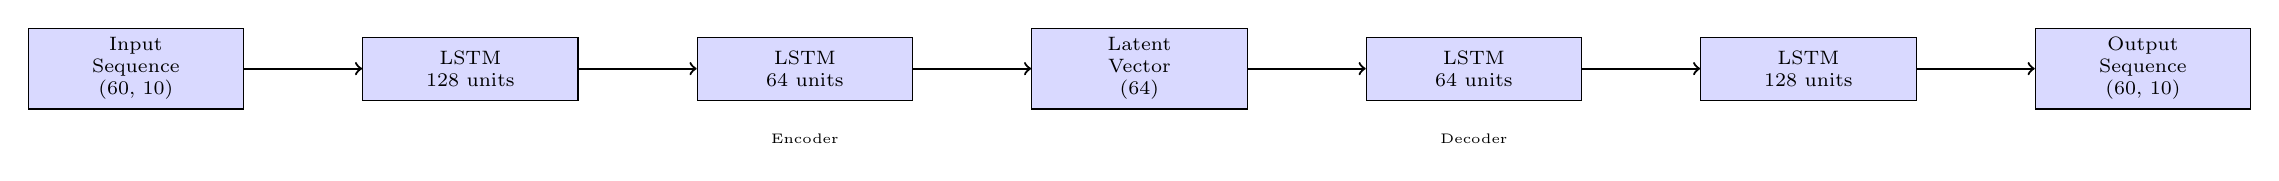
\begin{tikzpicture}[
    node distance=1.5cm,
    layer/.style={rectangle, draw, fill=blue!15, text width=2.5cm, align=center, minimum height=0.8cm, font=\scriptsize}
]

\node[layer] (input) {Input\\Sequence\\(60, 10)};
\node[layer, right=of input] (lstm1) {LSTM\\128 units};
\node[layer, right=of lstm1] (lstm2) {LSTM\\64 units};
\node[layer, right=of lstm2] (latent) {Latent\\Vector\\(64)};
\node[layer, right=of latent] (lstm3) {LSTM\\64 units};
\node[layer, right=of lstm3] (lstm4) {LSTM\\128 units};
\node[layer, right=of lstm4] (output) {Output\\Sequence\\(60, 10)};

\draw[->, thick] (input) -- (lstm1);
\draw[->, thick] (lstm1) -- (lstm2);
\draw[->, thick] (lstm2) -- (latent);
\draw[->, thick] (latent) -- (lstm3);
\draw[->, thick] (lstm3) -- (lstm4);
\draw[->, thick] (lstm4) -- (output);

\node[below=0.3cm of lstm2, font=\tiny] {Encoder};
\node[below=0.3cm of lstm3, font=\tiny] {Decoder};

\end{tikzpicture}
\caption{LSTM Autoencoder Architecture}
\end{figure}

\textbf{Responsibilities:}
\begin{itemize}[leftmargin=1cm,itemsep=0pt]
    \item Subscribe to sensor data from Kafka
    \item Create 60-second sliding windows
    \item Compute reconstruction error
    \item Flag anomalies (error > threshold)
    \item Publish alerts to Kafka
\end{itemize}

\textbf{Technology:} Python 3.11+, TensorFlow 2.x

\textbf{Federated:} Yes - Model weights shared across facilities

\subsubsection{Isolation Forest Component}

\textbf{Purpose:} Detect point anomalies (sudden outliers)

\textbf{Responsibilities:}
\begin{itemize}[leftmargin=1cm,itemsep=0pt]
    \item Subscribe to sensor and protocol data
    \item Compute anomaly scores
    \item Flag outliers (score > threshold)
    \item Publish alerts to Kafka
\end{itemize}

\textbf{Technology:} Python 3.11+, scikit-learn

\textbf{Federated:} Yes - Ensemble of trees shared

\subsubsection{Physics Rules Engine}

\textbf{Purpose:} Validate process physics constraints

\textbf{Responsibilities:}
\begin{itemize}[leftmargin=1cm,itemsep=0pt]
    \item Load facility-specific rules
    \item Evaluate rules against sensor data
    \item Detect violations (out of bounds, impossible rates)
    \item Publish violations to Kafka
\end{itemize}

\textbf{Technology:} Python 3.11+, custom rule engine

\textbf{Rule Types:}
\begin{itemize}[leftmargin=1cm,itemsep=0pt]
    \item \textbf{Range:} value must be in [min, max]
    \item \textbf{Rate:} change rate must be < max\_rate
    \item \textbf{Dependency:} if A then B must be true
    \item \textbf{Safety:} critical safety constraints
\end{itemize}

\textbf{Federated:} No - Rules are facility-specific


\subsubsection{Correlation Engine}

\textbf{Purpose:} Combine signals from multiple detection sources

\textbf{Architecture:}

\begin{figure}[H]
\centering
\begin{tikzpicture}[
    node distance=1cm,
    source/.style={rectangle, draw, fill=yellow!20, text width=2cm, align=center, minimum height=0.7cm, font=\scriptsize},
    engine/.style={rectangle, draw, fill=orange!20, text width=3cm, align=center, minimum height=1.5cm, font=\small},
    output/.style={rectangle, draw, fill=green!20, text width=2.5cm, align=center, minimum height=0.7cm, font=\scriptsize}
]

\node[source] (lstm) {LSTM\\Anomalies};
\node[source, below=0.5cm of lstm] (if) {Isolation\\Forest};
\node[source, below=0.5cm of if] (physics) {Physics\\Violations};
\node[source, below=0.5cm of physics] (protocol) {Protocol\\Anomalies};

\node[engine, right=2cm of if, yshift=-0.5cm] (corr) {Correlation\\Engine\\\\Temporal\\Spatial\\Severity};

\node[output, right=2cm of corr, yshift=0.5cm] (alert) {Unified\\Alert};
\node[output, below=0.5cm of alert] (incident) {Incident\\Report};

\draw[->, thick] (lstm) -- (corr);
\draw[->, thick] (if) -- (corr);
\draw[->, thick] (physics) -- (corr);
\draw[->, thick] (protocol) -- (corr);
\draw[->, thick] (corr) -- (alert);
\draw[->, thick] (corr) -- (incident);

\end{tikzpicture}
\caption{Correlation Engine - Multi-Source Fusion}
\end{figure}

\textbf{Responsibilities:}
\begin{itemize}[leftmargin=1cm,itemsep=0pt]
    \item Subscribe to all alert topics
    \item Temporal correlation (events within time window)
    \item Spatial correlation (events on related assets)
    \item Severity scoring (combine confidence scores)
    \item Generate unified threat assessments
    \item Publish to alerts.critical or alerts.warning
\end{itemize}

\textbf{Technology:} Python 3.11+, custom correlation logic

\subsubsection{Attack Prediction GNN}

\textbf{Purpose:} Predict attacker's next move using graph neural networks

\textbf{Architecture:}

\begin{figure}[H]
\centering
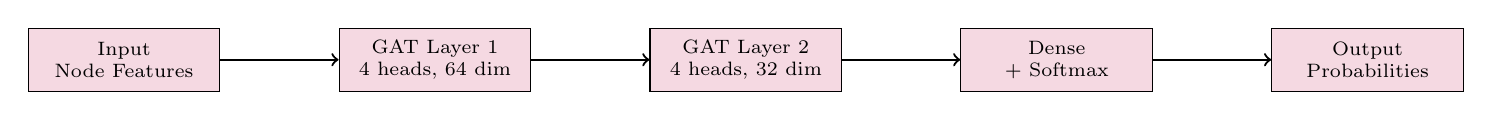
\begin{tikzpicture}[
    node distance=1.5cm,
    layer/.style={rectangle, draw, fill=purple!15, text width=2.2cm, align=center, minimum height=0.8cm, font=\scriptsize}
]

\node[layer] (input) {Input\\Node Features};
\node[layer, right=of input] (gat1) {GAT Layer 1\\4 heads, 64 dim};
\node[layer, right=of gat1] (gat2) {GAT Layer 2\\4 heads, 32 dim};
\node[layer, right=of gat2] (dense) {Dense\\+ Softmax};
\node[layer, right=of dense] (output) {Output\\Probabilities};

\draw[->, thick] (input) -- (gat1);
\draw[->, thick] (gat1) -- (gat2);
\draw[->, thick] (gat2) -- (dense);
\draw[->, thick] (dense) -- (output);

\end{tikzpicture}
\caption{Graph Attention Network for Attack Prediction}
\end{figure}

\textbf{Responsibilities:}
\begin{itemize}[leftmargin=1cm,itemsep=0pt]
    \item Load MITRE ATT\&CK graph from Neo4j
    \item Encode current attack state
    \item Predict next techniques with probabilities
    \item Publish predictions to Kafka
    \item Update graph with new attack chains
\end{itemize}

\textbf{Technology:} Python 3.11+, PyTorch, PyTorch Geometric

\textbf{Federated:} Yes - Learns attack chains from multiple facilities


\subsection{Federated Learning Layer}

\subsubsection{FL Architecture Overview}

\begin{figure}[H]
\centering
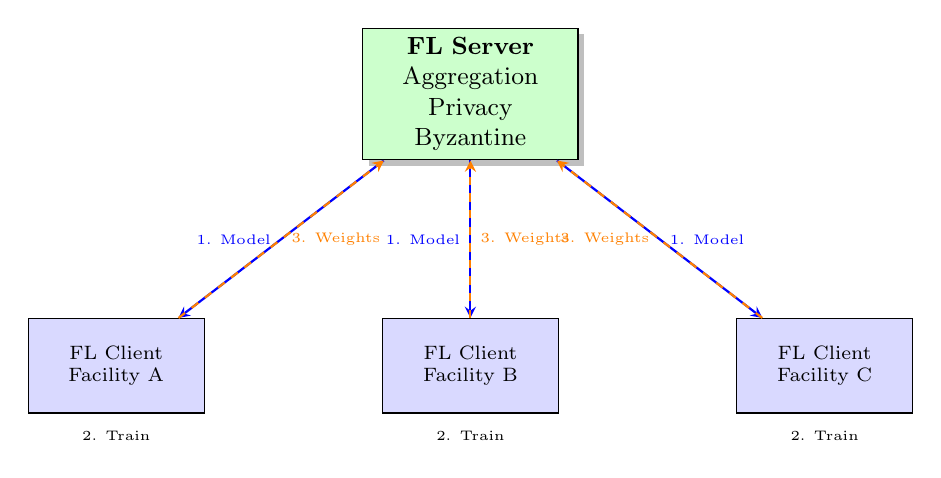
\begin{tikzpicture}[
    node distance=1.5cm,
    server/.style={rectangle, draw, fill=green!20, text width=2.5cm, align=center, minimum height=1.5cm, font=\small, drop shadow},
    client/.style={rectangle, draw, fill=blue!15, text width=2cm, align=center, minimum height=1.2cm, font=\scriptsize},
    arrow/.style={->, >=stealth, thick}
]

\node[server] (server) {\textbf{FL Server}\\Aggregation\\Privacy\\Byzantine};

\node[client, below left=2cm and 2cm of server] (c1) {FL Client\\Facility A};
\node[client, below=2cm of server] (c2) {FL Client\\Facility B};
\node[client, below right=2cm and 2cm of server] (c3) {FL Client\\Facility C};

\draw[arrow, color=blue] (server) -- node[left, font=\tiny] {1. Model} (c1);
\draw[arrow, color=blue] (server) -- node[left, font=\tiny] {1. Model} (c2);
\draw[arrow, color=blue] (server) -- node[right, font=\tiny] {1. Model} (c3);

\draw[arrow, color=orange, dashed] (c1) -- node[right, font=\tiny] {3. Weights} (server);
\draw[arrow, color=orange, dashed] (c2) -- node[right, font=\tiny] {3. Weights} (server);
\draw[arrow, color=orange, dashed] (c3) -- node[left, font=\tiny] {3. Weights} (server);

\node[below=0.1cm of c1, font=\tiny] {2. Train};
\node[below=0.1cm of c2, font=\tiny] {2. Train};
\node[below=0.1cm of c3, font=\tiny] {2. Train};

\end{tikzpicture}
\caption{Federated Learning Architecture - Server and Clients}
\end{figure}

\subsubsection{FL Client Component}

\textbf{Purpose:} Manage local training and weight transmission

\textbf{Responsibilities:}
\begin{itemize}[leftmargin=1cm,itemsep=0pt]
    \item Receive global model from FL server
    \item Train on local data (5 epochs)
    \item Compute weight updates
    \item Apply differential privacy noise
    \item Apply gradient clipping
    \item Send masked weights to server
    \item Deploy updated global model
\end{itemize}

\textbf{Technology:} Python 3.11+, Flower (flwr), TensorFlow/PyTorch

\textbf{Workflow:}
\begin{enumerate}[leftmargin=1cm,itemsep=0pt]
    \item Wait for FL round notification
    \item Download global model
    \item Load local training data
    \item Train for 5 epochs
    \item Compute weight deltas
    \item Apply gradient clipping (max\_norm=1.0)
    \item Add differential privacy noise
    \item Apply secure aggregation masks
    \item Upload to FL server
    \item Wait for next round
\end{enumerate}

\subsubsection{FL Server Component}

\textbf{Purpose:} Coordinate federated learning rounds and aggregate updates

\textbf{Responsibilities:}
\begin{itemize}[leftmargin=1cm,itemsep=0pt]
    \item Schedule FL rounds (4 per day)
    \item Distribute global model to clients
    \item Collect weight updates from clients
    \item Apply Byzantine-robust aggregation
    \item Compute new global model
    \item Distribute updated model
    \item Log metrics and monitor health
\end{itemize}

\textbf{Technology:} Python 3.11+, Flower (flwr), FastAPI

\textbf{Aggregation Algorithm:} Coordinate-wise median with outlier detection


\subsubsection{Privacy Engine}

\textbf{Purpose:} Apply differential privacy to weight updates

\textbf{Responsibilities:}
\begin{itemize}[leftmargin=1cm,itemsep=0pt]
    \item Generate calibrated noise
    \item Add noise to gradients/weights
    \item Track privacy budget
    \item Provide privacy guarantees
\end{itemize}

\textbf{Technology:} Python 3.11+, Opacus (PyTorch), TensorFlow Privacy

\textbf{Privacy Parameters:}
\begin{itemize}[leftmargin=1cm,itemsep=0pt]
    \item Epsilon (ε): 2.0 (moderate privacy)
    \item Delta (δ): 10⁻⁵ (failure probability)
    \item Noise mechanism: Gaussian
    \item Gradient clipping: L2 norm, max=1.0
\end{itemize}

\subsection{Storage Layer}

\textbf{Purpose:} Polyglot persistence for different data types

\subsubsection{Apache IoTDB}

\textbf{Purpose:} Store high-frequency sensor readings

\textbf{Technology:} Time-series database optimized for IoT workloads

\textbf{Key Features:}
\begin{itemize}[leftmargin=1cm,itemsep=0pt]
    \item High write throughput (1M points/second)
    \item Efficient compression (GORILLA encoding)
    \item Fast time-range queries
    \item Distributed architecture
\end{itemize}

\subsubsection{PostgreSQL}

\textbf{Purpose:} Store structured data (alerts, incidents, metadata)

\textbf{Technology:} Relational database with JSONB support

\textbf{Key Features:}
\begin{itemize}[leftmargin=1cm,itemsep=0pt]
    \item ACID transactions
    \item Complex queries and joins
    \item Full-text search
    \item Replication and high availability
\end{itemize}

\subsubsection{MongoDB}

\textbf{Purpose:} Store semi-structured logs and protocol messages

\textbf{Technology:} Document-oriented NoSQL database

\textbf{Key Features:}
\begin{itemize}[leftmargin=1cm,itemsep=0pt]
    \item Flexible schema
    \item High write throughput
    \item Horizontal scaling (sharding)
    \item Rich query language
\end{itemize}

\subsubsection{Neo4j}

\textbf{Purpose:} Store attack graphs and MITRE ATT\&CK relationships

\textbf{Technology:} Graph database

\textbf{Key Features:}
\begin{itemize}[leftmargin=1cm,itemsep=0pt]
    \item Native graph storage and processing
    \item Cypher query language
    \item Path finding algorithms
    \item Graph analytics
\end{itemize}


\subsection{API \& Presentation Layer}

\subsubsection{REST API}

\textbf{Purpose:} Provide standard CRUD operations

\textbf{Technology:} Python 3.11+, FastAPI

\textbf{Key Endpoints:}
\begin{itemize}[leftmargin=1cm,itemsep=0pt]
    \item \texttt{/api/alerts} - Alert management
    \item \texttt{/api/incidents} - Incident tracking
    \item \texttt{/api/facilities} - Facility configuration
    \item \texttt{/api/models} - Model management
    \item \texttt{/api/metrics} - System metrics
\end{itemize}

\textbf{Features:}
\begin{itemize}[leftmargin=1cm,itemsep=0pt]
    \item OpenAPI/Swagger documentation
    \item JWT authentication
    \item Rate limiting
    \item Request validation
\end{itemize}

\subsubsection{GraphQL API}

\textbf{Purpose:} Provide flexible, efficient queries

\textbf{Technology:} Python 3.11+, Strawberry GraphQL

\textbf{Key Features:}
\begin{itemize}[leftmargin=1cm,itemsep=0pt]
    \item Single endpoint for all queries
    \item Client-specified response structure
    \item Reduced over-fetching
    \item Real-time subscriptions
\end{itemize}

\subsubsection{WebSocket Service}

\textbf{Purpose:} Real-time updates to connected clients

\textbf{Technology:} Python 3.11+, FastAPI WebSockets

\textbf{Use Cases:}
\begin{itemize}[leftmargin=1cm,itemsep=0pt]
    \item Live alert notifications
    \item Real-time sensor data streaming
    \item System status updates
    \item FL training progress
\end{itemize}

\subsubsection{Web Dashboard}

\textbf{Purpose:} User interface for monitoring and management

\textbf{Technology:} React, TypeScript, Material-UI

\textbf{Key Views:}
\begin{itemize}[leftmargin=1cm,itemsep=0pt]
    \item Real-time threat dashboard
    \item Alert management console
    \item Incident response workflow
    \item System health monitoring
    \item FL training visualization
    \item Attack graph explorer
\end{itemize}

\section{Component Interactions}

\subsection{Data Flow}

\subsubsection{Normal Operation Flow}

\begin{enumerate}[leftmargin=1cm,itemsep=0pt]
    \item Protocol parsers capture ICS traffic
    \item Raw data published to Kafka topics
    \item Detection components consume from Kafka
    \item Anomalies detected and published as alerts
    \item Correlation engine fuses multi-source alerts
    \item Unified alerts stored in PostgreSQL
    \item WebSocket pushes alerts to dashboard
    \item Users review and respond via UI
\end{enumerate}

\subsubsection{Federated Learning Flow}

\begin{enumerate}[leftmargin=1cm,itemsep=0pt]
    \item FL Server schedules training round
    \item Global model distributed to clients
    \item Clients train on local data
    \item Privacy engine adds differential privacy noise
    \item Encrypted weights sent to server
    \item Server performs Byzantine-robust aggregation
    \item New global model computed
    \item Updated model distributed to all clients
    \item Clients deploy new model for inference
\end{enumerate}


\subsection{Attack Prediction Flow}

\begin{enumerate}[leftmargin=1cm,itemsep=0pt]
    \item Correlation engine detects attack technique
    \item Attack mapped to MITRE ATT\&CK framework
    \item GNN loads attack graph from Neo4j
    \item Current attack state encoded as node features
    \item GNN predicts next likely techniques
    \item Predictions published to Kafka
    \item Dashboard displays predicted attack path
    \item Recommended countermeasures generated
\end{enumerate}

\section{Security Architecture}

\subsection{Network Security}

\textbf{Segmentation:}
\begin{itemize}[leftmargin=1cm,itemsep=0pt]
    \item ICS network isolated from IT network
    \item DMZ for external API access
    \item Internal network for components
    \item Separate FL network for model updates
\end{itemize}

\textbf{Encryption:}
\begin{itemize}[leftmargin=1cm,itemsep=0pt]
    \item TLS 1.3 for all external communications
    \item mTLS for inter-service communication
    \item Encrypted Kafka topics for sensitive data
    \item Encrypted storage at rest
\end{itemize}

\subsection{Application Security}

\textbf{Authentication \& Authorization:}
\begin{itemize}[leftmargin=1cm,itemsep=0pt]
    \item JWT-based authentication
    \item Role-based access control (RBAC)
    \item Multi-factor authentication (MFA)
    \item API key management
\end{itemize}

\textbf{Input Validation:}
\begin{itemize}[leftmargin=1cm,itemsep=0pt]
    \item Schema validation for all inputs
    \item Sanitization of user inputs
    \item Rate limiting and throttling
    \item DDoS protection
\end{itemize}

\subsection{Privacy Architecture}

\textbf{Differential Privacy:}
\begin{itemize}[leftmargin=1cm,itemsep=0pt]
    \item Gaussian noise added to gradients
    \item Privacy budget tracking (ε=2.0, δ=10⁻⁵)
    \item Gradient clipping for bounded sensitivity
    \item Per-facility privacy accounting
\end{itemize}

\textbf{Secure Aggregation:}
\begin{itemize}[leftmargin=1cm,itemsep=0pt]
    \item Encrypted weight updates
    \item Server cannot see individual updates
    \item Byzantine-robust aggregation
    \item Outlier detection and filtering
\end{itemize}

\textbf{Data Minimization:}
\begin{itemize}[leftmargin=1cm,itemsep=0pt]
    \item Raw data never leaves facility
    \item Only model weights shared
    \item Aggregated statistics only
    \item Automatic data retention policies
\end{itemize}

\section{Scalability Architecture}

\subsection{Horizontal Scaling}

\textbf{Stateless Components:}
\begin{itemize}[leftmargin=1cm,itemsep=0pt]
    \item API servers (scale with load balancer)
    \item Detection components (scale with Kafka partitions)
    \item Protocol parsers (scale per data source)
\end{itemize}

\textbf{Stateful Components:}
\begin{itemize}[leftmargin=1cm,itemsep=0pt]
    \item Kafka brokers (add brokers, rebalance)
    \item Database sharding (PostgreSQL, MongoDB)
    \item IoTDB cluster expansion
    \item Neo4j clustering
\end{itemize}


\subsection{Load Balancing}

\textbf{API Layer:}
\begin{itemize}[leftmargin=1cm,itemsep=0pt]
    \item Nginx/HAProxy for HTTP load balancing
    \item Round-robin with health checks
    \item Session affinity for WebSockets
\end{itemize}

\textbf{Kafka:}
\begin{itemize}[leftmargin=1cm,itemsep=0pt]
    \item Partition-based load distribution
    \item Consumer groups for parallel processing
    \item Automatic rebalancing on failures
\end{itemize}

\subsection{Caching Strategy}

\textbf{Application Cache:}
\begin{itemize}[leftmargin=1cm,itemsep=0pt]
    \item Redis for session data
    \item Model weights caching
    \item Frequently accessed alerts
    \item System configuration
\end{itemize}

\textbf{Database Query Cache:}
\begin{itemize}[leftmargin=1cm,itemsep=0pt]
    \item PostgreSQL query result cache
    \item MongoDB in-memory cache
    \item IoTDB query cache
\end{itemize}

\section{Resilience Architecture}

\subsection{Fault Tolerance}

\textbf{Component Redundancy:}
\begin{itemize}[leftmargin=1cm,itemsep=0pt]
    \item Multiple instances of each service
    \item Active-active for stateless components
    \item Active-passive for stateful components
    \item Automatic failover mechanisms
\end{itemize}

\textbf{Data Replication:}
\begin{itemize}[leftmargin=1cm,itemsep=0pt]
    \item Kafka replication factor: 3
    \item PostgreSQL streaming replication
    \item MongoDB replica sets
    \item IoTDB data replication
\end{itemize}

\subsection{Graceful Degradation}

\textbf{Failure Modes:}
\begin{itemize}[leftmargin=1cm,itemsep=0pt]
    \item If FL unavailable: use local models
    \item If Kafka unavailable: buffer locally
    \item If database unavailable: cache in memory
    \item If detection component fails: others continue
\end{itemize}

\textbf{Circuit Breakers:}
\begin{itemize}[leftmargin=1cm,itemsep=0pt]
    \item Automatic service isolation on failures
    \item Exponential backoff for retries
    \item Fallback to cached data
    \item Health check endpoints
\end{itemize}

\subsection{Disaster Recovery}

\textbf{Backup Strategy:}
\begin{itemize}[leftmargin=1cm,itemsep=0pt]
    \item Automated daily backups
    \item Point-in-time recovery capability
    \item Off-site backup storage
    \item Regular restore testing
\end{itemize}

\textbf{Recovery Procedures:}
\begin{itemize}[leftmargin=1cm,itemsep=0pt]
    \item Documented recovery playbooks
    \item Automated recovery scripts
    \item Recovery time objective (RTO): 4 hours
    \item Recovery point objective (RPO): 1 hour
\end{itemize}


\section{Monitoring \& Observability}

\subsection{Metrics Collection}

\textbf{System Metrics:}
\begin{itemize}[leftmargin=1cm,itemsep=0pt]
    \item CPU, memory, disk, network utilization
    \item Service health and availability
    \item Request rates and latencies
    \item Error rates and types
\end{itemize}

\textbf{Application Metrics:}
\begin{itemize}[leftmargin=1cm,itemsep=0pt]
    \item Detection accuracy and false positive rates
    \item Alert generation rates
    \item FL training progress and convergence
    \item Model inference latencies
\end{itemize}

\textbf{Business Metrics:}
\begin{itemize}[leftmargin=1cm,itemsep=0pt]
    \item Threats detected per day
    \item Mean time to detect (MTTD)
    \item Mean time to respond (MTTR)
    \item Facility participation in FL
\end{itemize}

\subsection{Logging}

\textbf{Structured Logging:}
\begin{itemize}[leftmargin=1cm,itemsep=0pt]
    \item JSON format for all logs
    \item Correlation IDs for request tracing
    \item Log levels: DEBUG, INFO, WARN, ERROR, CRITICAL
    \item Centralized log aggregation
\end{itemize}

\textbf{Log Categories:}
\begin{itemize}[leftmargin=1cm,itemsep=0pt]
    \item Application logs
    \item Access logs
    \item Audit logs
    \item Security logs
\end{itemize}

\subsection{Distributed Tracing}

\textbf{Trace Propagation:}
\begin{itemize}[leftmargin=1cm,itemsep=0pt]
    \item OpenTelemetry instrumentation
    \item Trace context propagation across services
    \item Span creation for key operations
    \item Performance bottleneck identification
\end{itemize}

\subsection{Alerting}

\textbf{Alert Conditions:}
\begin{itemize}[leftmargin=1cm,itemsep=0pt]
    \item Service downtime or degradation
    \item High error rates
    \item Resource exhaustion
    \item Security events
    \item FL training failures
\end{itemize}

\textbf{Alert Channels:}
\begin{itemize}[leftmargin=1cm,itemsep=0pt]
    \item Email notifications
    \item SMS for critical alerts
    \item Slack/Teams integration
    \item PagerDuty for on-call
\end{itemize}

\section{Deployment Architecture}

\subsection{Containerization}

\textbf{Container Strategy:}
\begin{itemize}[leftmargin=1cm,itemsep=0pt]
    \item Docker containers for all services
    \item Multi-stage builds for optimization
    \item Base images with security patches
    \item Container registry for image storage
\end{itemize}

\subsection{Orchestration}

\textbf{Kubernetes Deployment:}
\begin{itemize}[leftmargin=1cm,itemsep=0pt]
    \item Kubernetes for container orchestration
    \item Helm charts for deployment management
    \item Namespaces for environment isolation
    \item Resource limits and requests
    \item Auto-scaling policies
\end{itemize}


\subsection{Infrastructure}

\textbf{Deployment Options:}
\begin{itemize}[leftmargin=1cm,itemsep=0pt]
    \item On-premises deployment for sensitive facilities
    \item Private cloud for hybrid deployments
    \item Edge computing for protocol parsers
    \item Centralized FL server in secure location
\end{itemize}

\textbf{Network Architecture:}
\begin{itemize}[leftmargin=1cm,itemsep=0pt]
    \item VPN tunnels between facilities
    \item Firewall rules for service isolation
    \item Network segmentation (ICS, DMZ, internal)
    \item DDoS protection at network edge
\end{itemize}

\section{Technology Stack Summary}

\subsection{Core Technologies}

\textbf{Programming Languages:}
\begin{itemize}[leftmargin=1cm,itemsep=0pt]
    \item Python 3.11+ (backend services, ML models)
    \item TypeScript (frontend dashboard)
    \item SQL (database queries)
    \item Cypher (graph queries)
\end{itemize}

\textbf{Machine Learning Frameworks:}
\begin{itemize}[leftmargin=1cm,itemsep=0pt]
    \item TensorFlow 2.x (LSTM Autoencoder)
    \item PyTorch (GNN, general deep learning)
    \item scikit-learn (Isolation Forest, preprocessing)
    \item PyTorch Geometric (graph neural networks)
\end{itemize}

\textbf{Federated Learning:}
\begin{itemize}[leftmargin=1cm,itemsep=0pt]
    \item Flower (flwr) - FL framework
    \item Opacus - differential privacy for PyTorch
    \item TensorFlow Privacy - differential privacy for TensorFlow
\end{itemize}

\textbf{Web Frameworks:}
\begin{itemize}[leftmargin=1cm,itemsep=0pt]
    \item FastAPI (REST API, WebSockets)
    \item Strawberry GraphQL (GraphQL API)
    \item React (frontend dashboard)
    \item Material-UI (UI components)
\end{itemize}

\textbf{Message Broker:}
\begin{itemize}[leftmargin=1cm,itemsep=0pt]
    \item Apache Kafka (distributed streaming)
    \item Kafka Connect (data integration)
    \item Kafka Streams (stream processing)
\end{itemize}

\textbf{Databases:}
\begin{itemize}[leftmargin=1cm,itemsep=0pt]
    \item Apache IoTDB (time-series)
    \item PostgreSQL (relational)
    \item MongoDB (document)
    \item Neo4j (graph)
    \item Redis (cache)
\end{itemize}

\textbf{Infrastructure:}
\begin{itemize}[leftmargin=1cm,itemsep=0pt]
    \item Docker (containerization)
    \item Kubernetes (orchestration)
    \item Helm (package management)
    \item Nginx (load balancing, reverse proxy)
\end{itemize}

\textbf{Monitoring \& Observability:}
\begin{itemize}[leftmargin=1cm,itemsep=0pt]
    \item Prometheus (metrics collection)
    \item Grafana (visualization)
    \item ELK Stack (logging: Elasticsearch, Logstash, Kibana)
    \item Jaeger (distributed tracing)
    \item OpenTelemetry (instrumentation)
\end{itemize}


\section{Design Patterns}

\subsection{Architectural Patterns}

\textbf{Microservices Architecture:}
\begin{itemize}[leftmargin=1cm,itemsep=0pt]
    \item Loosely coupled, independently deployable services
    \item Service-per-component design
    \item API gateway for external access
    \item Service mesh for inter-service communication
\end{itemize}

\textbf{Event-Driven Architecture:}
\begin{itemize}[leftmargin=1cm,itemsep=0pt]
    \item Kafka as central event bus
    \item Asynchronous communication between components
    \item Event sourcing for audit trails
    \item CQRS (Command Query Responsibility Segregation)
\end{itemize}

\textbf{Layered Architecture:}
\begin{itemize}[leftmargin=1cm,itemsep=0pt]
    \item Clear separation of concerns
    \item Data sources → Messaging → Processing → Storage → API
    \item Each layer depends only on layers below
    \item Horizontal scalability at each layer
\end{itemize}

\subsection{Design Patterns}

\textbf{Producer-Consumer Pattern:}
\begin{itemize}[leftmargin=1cm,itemsep=0pt]
    \item Protocol parsers as producers
    \item Detection components as consumers
    \item Kafka topics as queues
    \item Decoupled, scalable processing
\end{itemize}

\textbf{Observer Pattern:}
\begin{itemize}[leftmargin=1cm,itemsep=0pt]
    \item WebSocket clients observe alert stream
    \item Dashboard updates on new events
    \item Real-time notification system
\end{itemize}

\textbf{Strategy Pattern:}
\begin{itemize}[leftmargin=1cm,itemsep=0pt]
    \item Multiple detection algorithms (LSTM, IF, Physics)
    \item Pluggable aggregation strategies
    \item Configurable privacy mechanisms
\end{itemize}

\textbf{Repository Pattern:}
\begin{itemize}[leftmargin=1cm,itemsep=0pt]
    \item Abstract data access layer
    \item Database-agnostic business logic
    \item Testable data operations
\end{itemize}

\textbf{Circuit Breaker Pattern:}
\begin{itemize}[leftmargin=1cm,itemsep=0pt]
    \item Prevent cascading failures
    \item Automatic service isolation
    \item Graceful degradation
\end{itemize}

\section{Quality Attributes}

\subsection{Performance}

\textbf{Latency Requirements:}
\begin{itemize}[leftmargin=1cm,itemsep=0pt]
    \item Alert detection: <30 seconds end-to-end
    \item API response time: <200ms (p95)
    \item Model inference: <100ms per sample
    \item Dashboard updates: <1 second
\end{itemize}

\textbf{Throughput Requirements:}
\begin{itemize}[leftmargin=1cm,itemsep=0pt]
    \item Kafka: 100,000 messages/second
    \item IoTDB: 1M data points/second
    \item API: 10,000 requests/second
\end{itemize}

\subsection{Reliability}

\textbf{Availability:}
\begin{itemize}[leftmargin=1cm,itemsep=0pt]
    \item System availability: 99.9\% (8.76 hours downtime/year)
    \item Detection components: 99.95\%
    \item API layer: 99.99\%
\end{itemize}

\textbf{Fault Tolerance:}
\begin{itemize}[leftmargin=1cm,itemsep=0pt]
    \item Survive single component failure
    \item Automatic failover <30 seconds
    \item No data loss on component failure
\end{itemize}


\subsection{Security}

\textbf{Confidentiality:}
\begin{itemize}[leftmargin=1cm,itemsep=0pt]
    \item Data encrypted in transit (TLS 1.3)
    \item Data encrypted at rest (AES-256)
    \item Differential privacy guarantees (ε=2.0)
    \item Access control on all resources
\end{itemize}

\textbf{Integrity:}
\begin{itemize}[leftmargin=1cm,itemsep=0pt]
    \item Cryptographic signatures for model updates
    \item Byzantine-robust aggregation
    \item Audit logs for all changes
    \item Input validation and sanitization
\end{itemize}

\textbf{Availability:}
\begin{itemize}[leftmargin=1cm,itemsep=0pt]
    \item DDoS protection
    \item Rate limiting
    \item Resource quotas
    \item Redundancy and failover
\end{itemize}

\subsection{Maintainability}

\textbf{Modularity:}
\begin{itemize}[leftmargin=1cm,itemsep=0pt]
    \item Clear component boundaries
    \item Well-defined interfaces
    \item Minimal coupling between services
    \item High cohesion within services
\end{itemize}

\textbf{Testability:}
\begin{itemize}[leftmargin=1cm,itemsep=0pt]
    \item Unit tests for all components
    \item Integration tests for workflows
    \item End-to-end tests for critical paths
    \item Mock services for testing
\end{itemize}

\textbf{Documentation:}
\begin{itemize}[leftmargin=1cm,itemsep=0pt]
    \item Architecture documentation (this document)
    \item API documentation (OpenAPI/Swagger)
    \item Code documentation (docstrings)
    \item Deployment guides
    \item Runbooks for operations
\end{itemize}

\subsection{Scalability}

\textbf{Horizontal Scaling:}
\begin{itemize}[leftmargin=1cm,itemsep=0pt]
    \item All stateless components scale horizontally
    \item Kafka partitioning for parallel processing
    \item Database sharding for data distribution
    \item Load balancing across instances
\end{itemize}

\textbf{Capacity Planning:}
\begin{itemize}[leftmargin=1cm,itemsep=0pt]
    \item Support 10-1000 facilities
    \item 1000-10000 sensors per facility
    \item 1-10 alerts per facility per day
    \item 4 FL rounds per day
\end{itemize}

\section{Future Enhancements}

\subsection{Planned Features}

\textbf{Advanced ML Models:}
\begin{itemize}[leftmargin=1cm,itemsep=0pt]
    \item Transformer-based anomaly detection
    \item Reinforcement learning for response automation
    \item Explainable AI for alert justification
    \item Transfer learning across facility types
\end{itemize}

\textbf{Enhanced Privacy:}
\begin{itemize}[leftmargin=1cm,itemsep=0pt]
    \item Homomorphic encryption for secure computation
    \item Secure multi-party computation
    \item Zero-knowledge proofs for verification
    \item Privacy-preserving data sharing protocols
\end{itemize}

\textbf{Extended Integrations:}
\begin{itemize}[leftmargin=1cm,itemsep=0pt]
    \item SIEM integration (Splunk, QRadar)
    \item SOAR platform integration
    \item Threat intelligence feeds
    \item Mobile applications (iOS, Android)
\end{itemize}

\textbf{Advanced Analytics:}
\begin{itemize}[leftmargin=1cm,itemsep=0pt]
    \item Predictive maintenance
    \item Root cause analysis
    \item Attack attribution
    \item Threat hunting tools
\end{itemize}

\end{document}
